\chapter{Lecture 02}
\hfill {\footnotesize \textit{Date: 09/02/2026}}

\begin{proposition}
    Let \(\mathbb{K}\) be a field. Then every ideal of \(\mathbb{K}[x]\) is principle, but it is not true in general in \(\mathbb{K}[x_1, \cdots, x_n]\) for \(n > 1\).
\end{proposition}
\begin{proof}
    We proceed similarly as in we did in the case of \(\mathbb{Z}\). But before that, we have to prove analogous Euclid's Division lemma for \(\mathbb{K}[x]\).
    \begin{claim}\label{claim:euclid_pol}
    Let \(f, g \in \mathbb{K}[x]\). If \(g \neq 0\), then there exists polynomials \(q, r \in \mathbb{K}[x]\) such \(f = gq + r\), where either \( r = 0 \) or \(\deg r < \deg g\).
\end{claim}

\begin{proof}[Proof of claim]
If \(g\) divides \(f\), then \(q = \frac{f}{g}\) and \( r = 0 \) works and we are done. If not, let \(r = f - gq\) be a polynomial of the least degree among all polynomials of the form \(f- lg\) with \(l \in \mathbb{K}[x]\). Then we must have \(\deg g > \deg r\). Otherwise, let the leading term of \(r\) and \(g\) be \(ax^m\) and \(bx^n\), respectively. Then \[r - g \cdot ab^{-1}x^{m-n} = f - gq - g \cdot ab^{-1}x^{m-n} = f - g(q + ab^{-1}x^{m-n})\] has smaller degree than \(r\) and is of the given form, which contradicts minimality of the degree of \(r\).
So, we have found \( q, r \in \mathbb{K} \) with  \( \operatorname{deg} g > \operatorname{deg} r\) such that  \( f = gq + r \).
\end{proof}

If \(\mathfrak{a}\) is an ideal of \(\mathbb{K}[x]\), we claim that \((g) = \mathfrak{a}\), where \(g\) is a polynomial of least positive degree in \(\mathfrak{a}\). Clearly, \((g) \subseteq \mathfrak{a}\). Let \(f \in \mathfrak{a}\), then by the~\autoref{claim:euclid_pol}, there exists \(q, r \in \mathbb{K}[x]\) such that \[f = gq + r, \quad \text{where} \deg r < \deg g.\] Here \(r = 0\), otherwise, \(r = f - gq \in \mathfrak{a}\), which contradicts the minimality of the degree of \(g\). Hence, \(f = gq \in (g) \), which implies \(\mathfrak{a} \subseteq (g)\). Therefore, \(\mathfrak{a} = (g)\).

However, in general, in \(\mathbb{K}[x_1, \cdots, x_n]\) for \(n > 1\), every ideal is not principle. As counter-example, we can consider the finitely generated ideal \((x_1, x_2)\).
\end{proof}

\section{Quotient Ring}
\begin{definition}[Quotient Ring]
    Suppose \(R\) is a (commutative) ring (with identity), and suppose \(\mathfrak{a}\) is an ideal of \(R\). So, \(\mathfrak{a}\) is an additive subgroup of the abelian group \((R, +)\)\footnote{For an abelian group, every subgroup \(H\) is normal, \(r + H = H + r\).}. \(R/\mathfrak{a}\) is a quotient group where elements look like \(r + \mathfrak{a}\). Define multiplication on \(R/\mathfrak{a}\): \[(r + \mathfrak{a}) \cdot (r' + \mathfrak{a}) = rr' + \mathfrak{a}.\] Then \((R/\mathfrak{a}, +, \cdot)\) becomes a ring called \emph{quotient ring} of \(R\) modulo \(\mathfrak{a}\).
\end{definition}
Since cosets of an additive group \((R, +)\) can have multiple representatives, we have to check well-definedness of the multiplication defined above, i.e., if \(r + \mathfrak{a} = h + \mathfrak{a}\) and \(r' + \mathfrak{a} = h' + \mathfrak{a}\), then \((r+\mathfrak{a}) \cdot (r'+\mathfrak{a}) = (h+\mathfrak{a})\cdot (h'+\mathfrak{a})\). Notice, \(r + \mathfrak{a} = h + \mathfrak{a}\) and \(r' + \mathfrak{a} = h' + \mathfrak{a} \Leftrightarrow r - h \in \mathfrak{a} \text{ and } r' - h' \in \mathfrak{a}\). Since \(\mathfrak{a}\) is an ideal, \[(r-h)r' \in \mathfrak{a} \implies rr' - hr' \in \mathfrak{a} \text{ and}\] \[h(r'-h') \in \mathfrak{a} \implies hr' - hh' \in \mathfrak{a}.\]
Since \(\mathfrak{a}\) is an additive subgroup,
\begin{align*}
    &(rr' - hr') + (hr' -hh') \in \mathfrak{a}\\
    \implies &rr' + (-hr' + hr') -hh' \in \mathfrak{a}\\
    \implies &rr' - hh' \in \mathfrak{a}\\
    \implies &rr' + \mathfrak{a} = hh' + \mathfrak{a}\\
    \therefore &(r+\mathfrak{a}) \cdot (r'+\mathfrak{a}) = (h + \mathfrak{a}) \cdot (h' + \mathfrak{a}).
\end{align*}
Associativity, distributive property, existence of identity (which is \(0 + \mathfrak{a} = \mathfrak{a}\)) and commutativity of \((R/\mathfrak{a}, +, \cdot)\) are routine checks.
\begin{ques}
    Can we take quotient modulo an ideal of a non-commutative ring?
\end{ques}
\begin{answer}[Instructor]
    Yes, we can! In that case, the ideal should be two-sided ideal. Recall, in a non-commutative ring \(R\), an additive subgroup \(\mathfrak{a}\) of \(R\) is called a \emph{left ideal} if \(R\mathfrak{a} \subseteq \mathfrak{a}\) and \emph{right ideal} if \(\mathfrak{a}R \subseteq \mathfrak{a}\). If \(\mathfrak{a}\) is both left and right ideal, then we call it a \emph{two-sided ideal}. For a two-sided ideal, the arguments given above work without any issues. See \autoref{example:cliffordalgebra}.
\end{answer}
\begin{example}[Clifford Algebra]\label{example:cliffordalgebra}
    Suppose \(\mathcal{V}\) is a vector space over \(\mathbb{K}\). Then its tensor algebra over \(\mathbb{K}\) is \[T(\mathcal{V}) = \bigoplus_{n\ge 0} \mathcal{V}^{\otimes n},\] where \(\mathcal{V}^{\otimes 0} := \mathbb{K}, \mathcal{V}^{\otimes 1}:= \mathcal{V}, \cdots, \mathcal{V}^{\otimes n}:= \mathcal{V} \otimes \cdots \otimes \mathcal{V} (n \text{ times)}\).

    \(T(\mathcal{V})\) is a ring with multiplicative identity given by \(1 \in \mathbb{K}\), which is non-commutative as \(x \otimes y \neq y \otimes x\). 

    Now, suppose \(Q\) is a non-degenerate bilinear form on \(\mathcal{V}\). Consider the ideal \[\mathfrak{a} = \langle v \otimes v - Q(v, v) \cdot 1\rangle_{v \in \mathcal{V}}.\] Here \(\mathfrak{a}\) is a two-sided ideal and \(T(\mathcal{V})/\mathfrak{a} =: \text{Clifford}(\mathcal{V}, Q)\) is called \emph{Clifford Algebra}, which is an example of a quotient ring of a non-commutative ring.
\end{example}
\begin{proposition}[Correspondence Theorem]\label{proposition:correspondencethm}
    Suppose \(R\) is a ring and \(I\) is is an ideal. Then there is an \(1-1\) order-preserving correspondence between the ideals of \(R\) containing \(I\) and the ideals of the quotient ring \(R/I\). The order-preserving \(1-1\) correspondence is given by: if \(J'\) is an ideal of \(R/I\), then the corresponding ideal in \(R\) is given by \(\pi^{-1}(J')\).\footnote{\(\pi\) is the canonical projection map that maps each element \(r\) of \(R\) to \(r+I\) in \(R/I\).}
\end{proposition}
\begin{proof}
    \begin{enumerate}[label= Step (\arabic*)., leftmargin=*]
        \item First we show that if \(J'\) is an ideal of the quotient \(R/I\), then \(\pi^{-1}(J')\) is an ideal in \(R\). 

        Firstly, \(0 \in \pi^{-1}(J')\), because \(\pi(0) = I \in J'\) as \(J'\) is an ideal of \(R/I\), so it must contain the additive identity \(I\) of \(R/I\).

        Suppose \(x, y \in \pi^{-1}(J')\). So \(\pi(x) = x + I, \pi(y) = y+I \in J'\). Since \(J'\) is an ideal, we have 
        \begin{align*}
            &(x+I) - (y+I) \in J'\\
            \implies &(x - y) + I \in J'\\
            \implies &\pi(x-y) \in J'\\
            \implies &(x-y) \in \pi^{-1}(J').
        \end{align*}
        Hence, using subgroup criterion, \(\pi^{-1}(J')\) is an additive subgroup of \(R\). 

    Also, if \(r \in R\), then \(r \cdot \pi^{-1}(J') \subseteq \pi^{-1}(J')\). To see that, suppose \(x \in \pi^{-1}(J')\), which implies \(x+I \in J'\), which implies \((r+I)(x+I) \in J'\) as \((r +I) \in R/I\), and that implies \[rx +I \in J' \implies \pi(rx) \in J' \implies rx \in \pi^{-1}(J').\]
    \(\therefore \pi^{-1}(J')\) is indeed an ideal of \(R\).
\item We want to show that if \(J'\) is an ideal of \(R/I\), then the ideal \(J = \pi^{-1}(J')\) of \(R\) contains \(I\). 

    Let \(x \in I\), then \(\pi(x) = I \in J'\), which implies \(x \in \pi^{-1}(J')\). Therefore, \(I \subseteq \pi^{-1}(J')\).

\item Lastly, we wish to prove the correspondence is an order-preserving bijection. Define two maps \(\phi\) and \(\tilde{\phi}\) as follows: 

    
\tikzset{every picture/.style={line width=0.75pt}} %set default line width to 0.75pt        

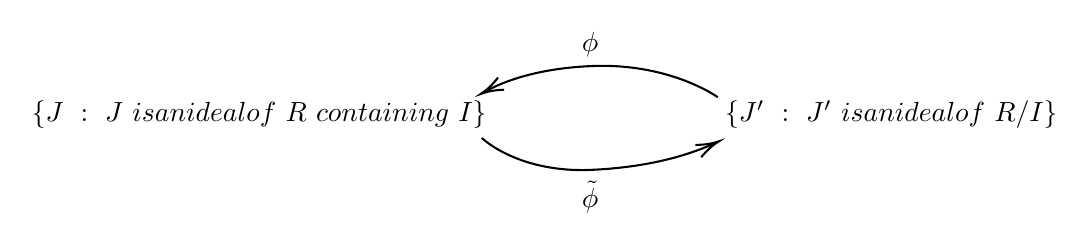
\begin{tikzpicture}[x=0.75pt,y=0.75pt,yscale=-1,xscale=1]
%uncomment if require: \path (0,300); %set diagram left start at 0, and has height of 300

%Curve Lines [id:da8286010344873176] 
\draw    (287.33,184.67) .. controls (288.08,185.42) and (305.5,201.5) .. (340,200) .. controls (372.09,198.61) and (391.3,190.94) .. (399.77,187.06) ;
\draw [shift={(401.5,186.25)}, rotate = 154.61] [color={rgb, 255:red, 0; green, 0; blue, 0 }  ][line width=0.75]    (10.93,-3.29) .. controls (6.95,-1.4) and (3.31,-0.3) .. (0,0) .. controls (3.31,0.3) and (6.95,1.4) .. (10.93,3.29)   ;
%Curve Lines [id:da6236228362848004] 
\draw    (288.6,162.44) .. controls (294.07,159.42) and (309.99,151.31) .. (340,150) .. controls (374.5,148.5) and (396.63,162) .. (401,165) ;
\draw [shift={(286.83,163.42)}, rotate = 333.09] [color={rgb, 255:red, 0; green, 0; blue, 0 }  ][line width=0.75]    (10.93,-3.29) .. controls (6.95,-1.4) and (3.31,-0.3) .. (0,0) .. controls (3.31,0.3) and (6.95,1.4) .. (10.93,3.29)   ;

% Text Node
\draw (69,165) node [anchor=north west][inner sep=0.75pt]    {$\left\{J\ :\ J\ \text{is an ideal of } \ R\ \text{containing} \ I\right\}$};
% Text Node
\draw (403,165) node [anchor=north west][inner sep=0.75pt]    {$\left\{J'\ :\ J'\ \text{is an ideal of } \ R/I\right\}$};
% Text Node
\draw (334,204) node [anchor=north west][inner sep=0.75pt]    {$\tilde{\phi }$};
% Text Node
\draw (334,132) node [anchor=north west][inner sep=0.75pt]    {$\phi $};
\end{tikzpicture}

\(\phi(J') = \pi^{-1}(J')\) and \(\tilde{\phi}(J) = \pi(J)\). We will prove \(\phi\) and \(\tilde{\phi}\) are inverses of each other and if \(J_1' \subseteq J_2'\), then \(\phi(J_1') \subseteq \phi(J_2')\).

Firstly, since \(\pi\) is surjective, \(\pi(\pi^{-1}(J')) = J'\), equivalently, \((\tilde{\phi} \circ \phi)(J') = J'\). For any set map, \( \pi^{-1}(\pi(J)) \supseteq J \) is true. And \( x \in \pi^{-1}(\pi(J)) \) implies \( \pi(x) \in \pi(J) \), which means there is an \( y \in J \) such that  \( \pi(x) = \pi(y) \), which implies \( \pi(x - y) = 0 \), and so \( (x - y) \in \operatorname{ker} \pi = I \subseteq J\). Here \( y \in J \), so is \( x = x - y + y \). Therefore, \( \pi^{-1}(\pi(J)) \subseteq J \), implying \( \pi^{-1}(\pi(J)) = J \), which is equivalent to \((\phi \circ \tilde{\phi})(J) = J\). So \(\phi\) and \(\tilde{\phi}\) are inverses of each other.

Furthermore, let \(x \in \phi(J_1') = \pi^{-1}(J_1')\). Then \(\pi(x) \in J_1' \subseteq J_2'\). So, \(x \in \pi^{-1}(J_2') = \phi(J_2')\). Hence, we have \(\phi(J_1') \subseteq \phi(J_2')\), completing the proof.
    \end{enumerate}
\end{proof}
\begin{definition}
    Let \(R\) be a ring.

    An element \(r \in R\) is called a \emph{zero-divisor} if there is a non-zero \(y \in R\) such that \(r \cdot y = 0\).

    \(R\) is called an \emph{integral domain} if it does not have any non-zero zero-divisors.

An element \(r \in R\) is called \emph{nilpotent} if \(r^n = 0\) for some \(n > 0\).

A \emph{unit} \(r \in R\) is an element that ``divides \(1\)'', i.e., for which there exists \(y \in R, y \neq 0\) such that \(xy = 1\).

\(R\) is a \emph{field} if \(1 \neq 0\) and every non-zero element is a unit.
\end{definition}
\begin{remark}
    \begin{itemize}
        \item \(0\) is also a zero-divisor.
        \item Nilpotent elements are all zero-divisors. To see that, suppose \(r\) is a nilpotent element and \(r^n = 0\). If \(n = 1\), then \(r\) is trivially zero-divisor. Otherwise, we have \(r^{n-1} \in R\) such that \(r \cdot r^{n-1} = 0\).
        \item The set of all units of a ring \(R\) forms an abelian group under multiplication and it is denoted by \(R^\times\).
        \item A unit cannot be a zero-divisor in \(R \neq (0)\). Suppose \(x\) is a unit with \(xy = 1\). If \(x\) is also a zero-divisor, then \(sx = 0\) for some \(s \neq 0\). \[sx = 0 \implies (sx)y = 0y \implies s(xy) = 0 \implies s \cdot 1 = 0  \implies s = 0 \text{ (contradiction!}).\] So,
        \item A field is an integral domain.
    \end{itemize}
\end{remark}
\begin{proposition}
    Suppose \(R\) is a ring and \(R \neq (0)\). Then the following are equivalent:
    \begin{enumerate}
        \item \(R\) is a field.
        \item \(R\) only has two ideals: (0) and \((1)\).
        \item Every homomorphism\footnote{Remember we require \(f(1) = 1\) for a ring homomorphism \(f\).} of \(R\) to a non-zero ring is injective.
    \end{enumerate}
\end{proposition}
\begin{proof}
    \begin{itemize}
        \item (1) \(\implies\) (2). Suppose \(R\) is a field. That means, every non-zero element is a unit. Let \(\mathfrak{a}\) be an ideal of \(R\). If \(\mathfrak{a} = (0)\), we are done. Otherwise, there exists non-zero \(x \in \mathfrak{a} \subseteq R\). Hence, \(x\) is a unit, i.e., there exits \(y \in R\) such that \(xy = yx = 1\). Since \(\mathfrak{a}\) is an ideal, \(y \cdot x \in \mathfrak{a} \implies 1 \in \mathfrak{a} \implies \mathfrak{a} = (1) = R\).

        \item (2) \(\implies\) (3). Suppose \(R\) has only two ideals: \((0)\) and \((1)\). And let \(f: R \longrightarrow S \neq (0)\) be a ring homomorphism. \(\ker f\) is an ideal of \(R\), and it can be either \((0)\) or \((1)\) as per hypothesis. But \(\ker f \neq R\) since we at least have \(1_R \not\in \ker f\) by definition. Hence, \(\ker f = (0)\), which implies \(f\) is injective\footnote{Recall from the first course in algebra: A ring homomorphism is injective iff its kernel is \((0)\).}.
        
        \item (3) \(\implies\) (1). Suppose every homomorphism of \(R\) to a non-zero ring is injective. We want to show that \(R\) is a field, i.e., every non-zero element is a unit. Suppose there is an element \(x \in R\) which is not a unit. Then \((x)\ \neq (1)\) (because if it was \((1)\), then that would mean for some \(y\), \(y \cdot x = 1 \implies x\) is a unit). 

            Consider the canonical projection map \(\pi: R \to R/(x)\) for which \(\ker \pi = (x)\). Since \((x) \neq (1)\), i.e., since \((x) \neq R, R/(x) \neq (0)\). Since \(\pi\) is injective by the hypothesis, so \(\ker \pi = (0)\), which implies \((x) = (0) \implies x = 0\). Hence, the only non-unit in \(R\) is \(0\), and so every non-zero element should be a unit.
    \end{itemize}
\end{proof}
